\documentclass[12pt]{article}

\usepackage[margin=3cm]{geometry}
\usepackage{amsmath, amssymb, amsthm}
\usepackage{url}
\usepackage{graphicx}
\usepackage{eqlist}
\usepackage{uri}
\urisetup{doipre={https://doi.org/}}
\usepackage{natbib}
\usepackage{siunitx}
\usepackage{pythonhighlight}
\usepackage{comment}
\usepackage{caption}
\usepackage{tabularx}
\usepackage{tikz}
\usepackage{tasks}
\usepackage{xcolor}
\usepackage{oubraces}
\usepackage[inline]{enumitem}
\usepackage{titling}
\usepackage{tcolorbox}
\tcbuselibrary{breakable}
\usepackage{needspace}
\usepackage{fancyhdr}
\usepackage[font={small}, labelfont=bf]{caption}
\captionsetup{width=.7\textwidth, font=small}
\usepackage{hyperref}
\usepackage{forest}
\hypersetup{
    colorlinks=true,
    urlcolor=blue,
    % hidelinks=true,
    linkcolor=black,
    citecolor=black,
}
\usetikzlibrary{positioning} 
% set the float page fraction
\renewcommand{\floatpagefraction}{.8}

% Initialize line spacing to 1.5
\linespread{1.5}

% Define math operators
\DeclareMathOperator{\sgn}{sgn}
\DeclareMathOperator{\real}{Re}
\DeclareMathOperator{\imag}{Im}
\DeclareMathOperator{\Ei}{Ei}
\DeclareMathOperator{\E1}{E_1}
\DeclareMathOperator{\atan2}{atan2}
\DeclareMathOperator{\lcm}{lcm}
\DeclareMathOperator{\gcf}{gcf}

% Convenience commands for colored boxes
\newcommand{\rbox}[1]{\fcolorbox{red}{white}{#1}}
\newcommand{\bbox}[1]{\fcolorbox{blue}{white}{#1}}

% Convenience command for hidden boxed content
\newcommand{\hide}[1]{\boxed{\phantom{#1}}}

% Simple exercises environment using basic enumerate
\newcounter{exercisenum}
\newenvironment{exercises}{%
  \begin{tcolorbox}[colback=white,colframe=black,arc=0pt,breakable]
%   \noindent\textbf{Exercises}\par
  \begin{enumerate}[label=\arabic*),leftmargin=1cm,resume=exercises]
  \setcounter{enumi}{\value{exercisenum}}
}{%
  \setcounter{exercisenum}{\value{enumi}}
  \end{enumerate}
  \end{tcolorbox}
}

% Setup footer for first page only
\fancypagestyle{firstpage}{
  \fancyhf{}
  \fancyfoot[L]{\small FRACTIONS}
  \fancyfoot[R]{\small \quad Ewan Short \quad \today}
  \fancyfoot[C]{\small\thepage}
  \renewcommand{\headrulewidth}{0pt}
  \renewcommand{\footrulewidth}{0pt}
}

\begin{document}

\thispagestyle{firstpage}

\section{Fractions}
\begin{itemize}
\item
\underbar{Fractions} like $\frac{1}{2}$ are often used to represent portions of something, like pizza. Below are some fractions shown as shaded slices of a pizza.
\begin{center}
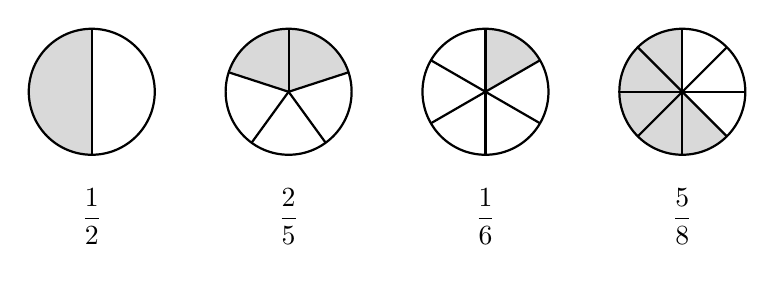
\begin{tikzpicture}

    % First pizza - divided in halves (1/2)
    \fill[gray!30] (0,0) -- (0,0.8) arc (90:270:0.8cm) -- cycle;
    \draw[thick] (0,0) circle (0.8cm);
    \draw[thick] (0,0.8) -- (0,-0.8);
    \node[anchor=base] at (0,-1.7) {$\displaystyle\frac{1}{2}$};
    
    % Second pizza - divided in fifths (2/5)
    \fill[gray!30] (2.5,0) -- (2.5,0.8) arc (90:162:0.8cm) -- cycle;
    \fill[gray!30] (2.5,0) -- (2.5,0.8) arc (90:18:0.8cm) -- cycle;
    \draw[thick] (2.5,0) circle (0.8cm);
    \foreach \angle in {90,162,234,306,18}
        \draw[thick] (2.5,0) -- ++(\angle:0.8cm);
    \node[anchor=base] at (2.5,-1.7) {$\displaystyle\frac{2}{5}$};
    
    % Third pizza - divided in sixths (1/6)
    \fill[gray!30] (5,0) -- (5,0.8) arc (90:30:0.8cm) -- cycle;
    \draw[thick] (5,0) circle (0.8cm);
    \foreach \angle in {90,150,210,270,330,30}
        \draw[thick] (5,0) -- ++(\angle:0.8cm);
    \node[anchor=base] at (5,-1.7) {$\displaystyle\frac{1}{6}$};
    
    % Fourth pizza - divided in eighths (4/8)
    \fill[gray!30] (7.5,0) -- (7.5,0.8) arc (90:315:0.8cm) -- cycle;
    \draw[thick] (7.5,0) circle (0.8cm);
    \foreach \angle in {90,135,180,225,270,315,0,45}
        \draw[thick] (7.5,0) -- ++(\angle:0.8cm);
    \node[anchor=base] at (7.5,-1.7) {$\displaystyle\frac{5}{8}$};
\end{tikzpicture}
\end{center}
\vspace{-1em}
\item
In a fraction, the number above the line is the \underbar{numerator}, which is the number of portions we have, or are interested in. The number below the line is the \underbar{denominator}, which is the total portions making up the whole.
$$
\frac{\text{portions}}{\text{total portions}} = \frac{\text{numerator}}{\text{denominator}} = \frac{\text{shaded slices}}{\text{total slices}}.
$$ 
\end{itemize}

\begin{exercises}
\item Shade the pizza slices and add the missing numbers as needed.
\begin{center}
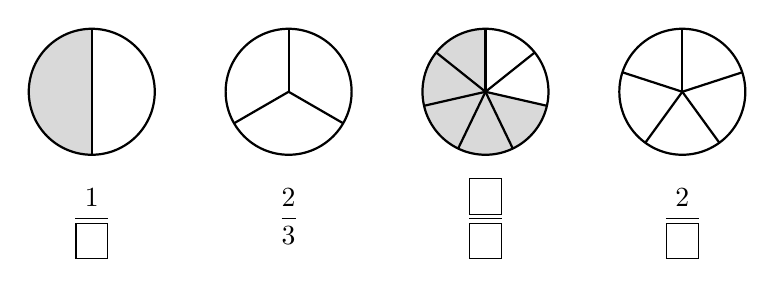
\begin{tikzpicture}
    % First pizza - divided in halves (1/2)
    \fill[gray!30] (0,0) -- (0,0.8) arc (90:270:0.8cm) -- cycle;
    \draw[thick] (0,0) circle (0.8cm);
    \draw[thick] (0,0.8) -- (0,-0.8);
    \node[anchor=base] at (0,-1.7) {$\displaystyle\frac{1}{\hide{2}}$};
    
    % Second pizza - divided in thirds (2/3)
    \draw[thick] (2.5,0) circle (0.8cm);
    \foreach \angle in {90,210,330}
        \draw[thick] (2.5,0) -- ++(\angle:0.8cm);
    \node[anchor=base] at (2.5,-1.7) {$\displaystyle\frac{2}{3}$};
    
    % Third pizza - divided in sevenths (5/7)
    \fill[gray!30] (5,0) -- (5,0.8) arc (90:347.14:0.8cm) -- cycle;
    \draw[thick] (5,0) circle (0.8cm);
    \foreach \angle in {90,141.43,192.86,244.29,295.71,347.14,38.57}
        \draw[thick] (5,0) -- ++(\angle:0.8cm);
    \node[anchor=base] at (5,-1.7) {$\displaystyle\frac{\hide{5}}{\hide{7}}$};
    
    % Fourth pizza - divided in fifths (2/5)
    \draw[thick] (7.5,0) circle (0.8cm);
    \foreach \angle in {90,162,234,306,18}
        \draw[thick] (7.5,0) -- ++(\angle:0.8cm);
    \node[anchor=base] at (7.5,-1.7) {$\displaystyle\frac{2}{\hide{5}}$};
\end{tikzpicture}
\end{center}
\end{exercises}

\begin{itemize}
\item
\underbar{Equivalent fractions} are different ways of writing the same fraction. Below is $\frac{1}{2}$ and some equivalent fractions.
\begin{center}
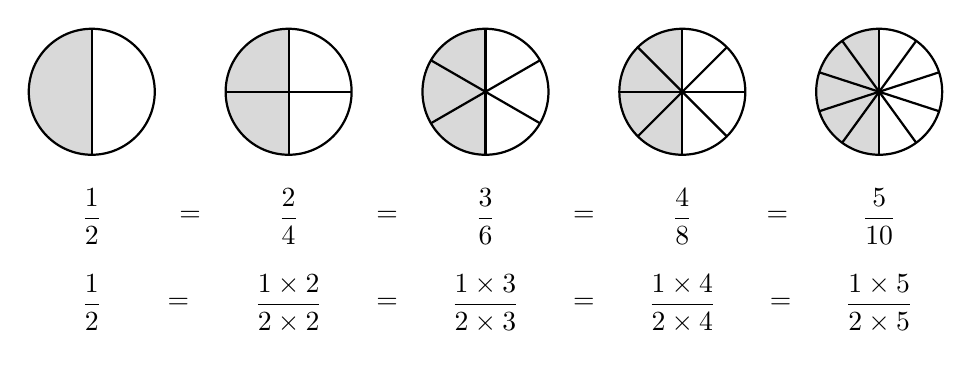
\begin{tikzpicture}
    % First pizza - divided in halves (1/2)
    \fill[gray!30] (0,0) -- (0,0.8) arc (90:270:0.8cm) -- cycle;
    \draw[thick] (0,0) circle (0.8cm);
    \draw[thick] (0,0.8) -- (0,-0.8);
    \node[anchor=base] (a) at (0,-1.7) {$\displaystyle\frac{1}{2}$};
    \node[anchor=north] (a2) at (0,-2.2) {$\displaystyle\frac{1}{2}$};
    
    % Second pizza - divided in quarters (2/4)
    \fill[gray!30] (2.5,0) -- (2.5,0.8) arc (90:270:0.8cm) -- cycle;
    \draw[thick] (2.5,0) circle (0.8cm);
    \draw[thick] (2.5,0.8) -- (2.5,-0.8);
    \draw[thick] (1.7,0) -- (3.3,0);
    \node[anchor=base] (b) at (2.5,-1.7) {$\displaystyle\frac{2}{4}$};
    \node[anchor=north] (b2) at (2.5,-2.2) {$\displaystyle\frac{1\times 2}{2\times 2}$};
    
    % Third pizza - divided in sixths (3/6)
    \fill[gray!30] (5,0) -- (5,0.8) arc (90:270:0.8cm) -- cycle;
    \draw[thick] (5,0) circle (0.8cm);
    \foreach \angle in {90,150,210,270,330,30}
        \draw[thick] (5,0) -- ++(\angle:0.8cm);
    \node[anchor=base] (c) at (5,-1.7) {$\displaystyle\frac{3}{6}$};
    \node[anchor=north] (c2) at (5,-2.2) {$\displaystyle\frac{1\times 3}{2\times 3}$};
    
    % Fourth pizza - divided in eighths (4/8)
    \fill[gray!30] (7.5,0) -- (7.5,0.8) arc (90:270:0.8cm) -- cycle;
    \draw[thick] (7.5,0) circle (0.8cm);
    \foreach \angle in {90,135,180,225,270,315,0,45}
        \draw[thick] (7.5,0) -- ++(\angle:0.8cm);
    \node[anchor=base] (d) at (7.5,-1.7) {$\displaystyle\frac{4}{8}$};
    \node[anchor=north] (d2) at (7.5,-2.2) {$\displaystyle\frac{1\times 4}{2\times 4}$};
    
    % Fifth pizza - divided in tenths (5/10)
    \fill[gray!30] (10,0) -- (10,0.8) arc (90:270:0.8cm) -- cycle;
    \draw[thick] (10,0) circle (0.8cm);
    \foreach \angle in {90,126,162,198,234,270,306,342,18,54}
        \draw[thick] (10,0) -- ++(\angle:0.8cm);
    \node[anchor=base] (e) at (10,-1.7) {$\displaystyle\frac{5}{10}$};
    \node[anchor=north] (e2) at (10,-2.2) {$\displaystyle\frac{1\times 5}{2\times 5}$};

    % Equals signs between top row
    \path (a) -- node[midway] {$=$} (b);
    \path (b) -- node[midway] {$=$} (c);
    \path (c) -- node[midway] {$=$} (d);
    \path (d) -- node[midway] {$=$} (e);
    
    % Equals signs between bottom row
    \path (a2) -- node[midway] {$=$} (b2);
    \path (b2) -- node[midway] {$=$} (c2);
    \path (c2) -- node[midway] {$=$} (d2);
    \path (d2) -- node[midway] {$=$} (e2);
\end{tikzpicture}
\end{center}
\item 
In the previous diagram, notice how multiplying the numerator and denominator by the same whole number creates equivalent fractions, and corresponds visually to subdividing the pizza slices.
\end{itemize}

\begin{exercises}
\item
Add the missing numbers to the equivalent fractions below.
\begin{center}
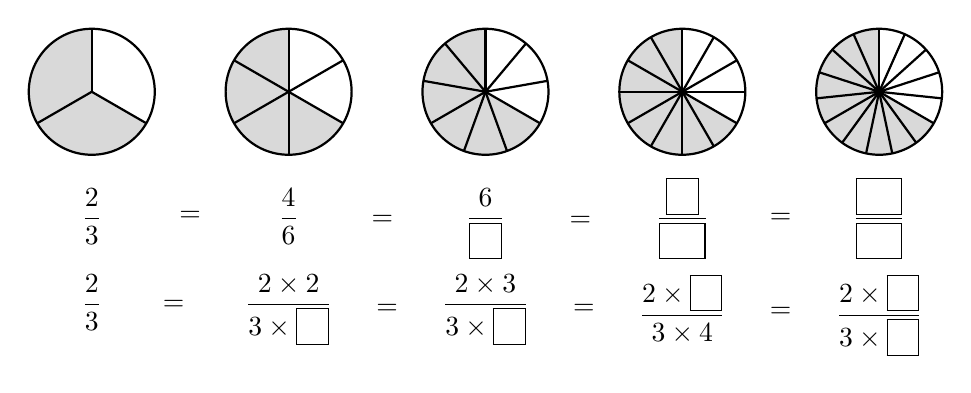
\begin{tikzpicture}
    % First pizza - divided in thirds (2/3)
    \fill[gray!30] (0,0) -- (0,0) -- ++(90:0.8cm) arc (90:330:0.8cm) -- cycle;
    \draw[thick] (0,0) circle (0.8cm);
    \foreach \angle in {90,210,330}
        \draw[thick] (0,0) -- ++(\angle:0.8cm);
    \node[anchor=base] (a) at (0,-1.7) {$\displaystyle\frac{2}{3}$};
    \node[anchor=north] (a2) at (0,-2.2) {$\displaystyle\frac{2}{3}$};
    
    % Second pizza - divided in sixths (4/6)
    \fill[gray!30] (2.5,0) -- (2.5,0) -- ++(90:0.8cm) arc (90:330:0.8cm) -- cycle;
    \draw[thick] (2.5,0) circle (0.8cm);
    \foreach \angle in {90,150,210,270,330,30}
        \draw[thick] (2.5,0) -- ++(\angle:0.8cm);
    \node[anchor=base] (b) at (2.5,-1.7) {$\displaystyle\frac{4}{6}$};
    \node[anchor=north] (b2) at (2.5,-2.2) {$\displaystyle\frac{2\times 2}{3\times \hide{2}}$};
    
    % Third pizza - divided in ninths (6/9)
    \fill[gray!30] (5,0) -- (5,0) -- ++(90:0.8cm) arc (90:330:0.8cm) -- cycle;
    \draw[thick] (5,0) circle (0.8cm);
    \foreach \angle in {90,130,170,210,250,290,330,10,50}
        \draw[thick] (5,0) -- ++(\angle:0.8cm);
    \node[anchor=base] (c) at (5,-1.7) {$\displaystyle\frac{6}{\hide{9}}$};
    \node[anchor=north] (c2) at (5,-2.2) {$\displaystyle\frac{2\times 3}{3\times \hide{3}}$};
    
    % Fourth pizza - divided in twelfths (8/12)
    \fill[gray!30] (7.5,0) -- (7.5,0) -- ++(90:0.8cm) arc (90:330:0.8cm) -- cycle;
    \draw[thick] (7.5,0) circle (0.8cm);
    \foreach \angle in {90,120,150,180,210,240,270,300,330,0,30,60}
        \draw[thick] (7.5,0) -- ++(\angle:0.8cm);
    \node[anchor=base] (d) at (7.5,-1.7) {$\displaystyle\frac{\hide{8}}{\hide{12}}$};
    \node[anchor=north] (d2) at (7.5,-2.2) {$\displaystyle\frac{2\times \hide{4}}{3\times 4}$};
    
    % Fifth pizza - divided in fifteenths (10/15)
    \fill[gray!30] (10,0) -- (10,0) -- ++(90:0.8cm) arc (90:330:0.8cm) -- cycle;
    \draw[thick] (10,0) circle (0.8cm);
    \foreach \angle in {90,114,138,162,186,210,234,258,282,306,330,354,18,42,66}
        \draw[thick] (10,0) -- ++(\angle:0.8cm);
    \node[anchor=base] (e) at (10,-1.7) {$\displaystyle\frac{\hide{10}}{\hide{15}}$};
    \node[anchor=north] (e2) at (10,-2.2) {$\displaystyle\frac{2\times \hide{5}}{3\times \hide{5}}$};

    % Equals signs between top row
    \path (a) -- node[midway] {$=$} (b);
    \path (b) -- node[midway] {$=$} (c);
    \path (c) -- node[midway] {$=$} (d);
    \path (d) -- node[midway] {$=$} (e);
    
    % Equals signs between bottom row
    \path (a2) -- node[midway] {$=$} (b2);
    \path (b2) -- node[midway] {$=$} (c2);
    \path (c2) -- node[midway] {$=$} (d2);
    \path (d2) -- node[midway] {$=$} (e2);
\end{tikzpicture}
\end{center}
\vspace{-1.5em}
\item
Find three fractions equivalent to $\frac{4}{7}$, for example $\frac{12}{21}$.
\end{exercises}

\section{Adding and Subtracting Fractions}
\begin{itemize}
\item
Fractions with the same denominator can be added or subtracted by adding or subtracting the numerators. For example,
\begin{center}
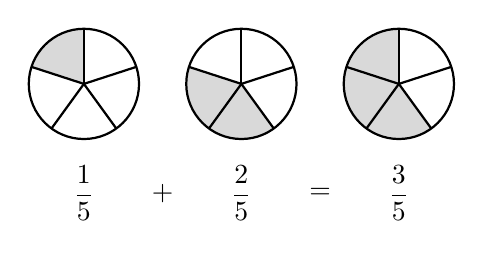
\begin{tikzpicture}
    % First pizza - 1/5
    \fill[gray!30] (0,0) -- (0,0.7) arc (90:162:0.7cm) -- cycle;
    \draw[thick] (0,0) circle (0.7cm);
    \foreach \angle in {90,162,234,306,18}
        \draw[thick] (0,0) -- ++(\angle:0.7cm);
    \node[anchor=base] (a) at (0,-1.5) {$\displaystyle\frac{1}{5}$};
    
    % Second pizza - 2/5
    \fill[gray!30] (2.0,0) -- ++(162:0.7cm) arc (162:306:0.7cm) -- cycle;
    \draw[thick] (2.0,0) circle (0.7cm);
    \foreach \angle in {90,162,234,306,18}
        \draw[thick] (2.0,0) -- ++(\angle:0.7cm);
    \node[anchor=base] (b) at (2.0,-1.5) {$\displaystyle\frac{2}{5}$};
    
    % Third pizza - 3/5
    \fill[gray!30] (4.0,0) -- (4.0,0.7) arc (90:306:0.7cm) -- cycle;
    \draw[thick] (4.0,0) circle (0.7cm);
    \foreach \angle in {90,162,234,306,18}
        \draw[thick] (4.0,0) -- ++(\angle:0.7cm);
    \node[anchor=base] (c) at (4.0,-1.5) {$\displaystyle\frac{3}{5}$};
    
    % Plus and equals signs between fractions
    \path (a) -- node[midway] {$\displaystyle+$} (b);
    \path (b) -- node[midway] {$\displaystyle=$} (c);
\end{tikzpicture}
\hspace{1.75cm}
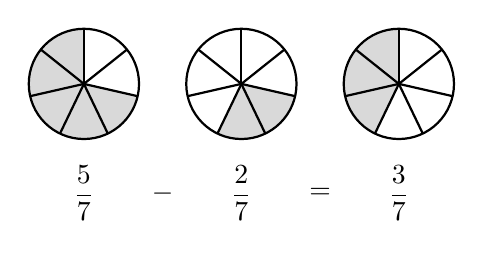
\begin{tikzpicture}
    % First pizza - 5/7
    \fill[gray!30] (0,0) -- (0,0.7) arc (90:347.14:0.7cm) -- cycle;
    \draw[thick] (0,0) circle (0.7cm);
    \foreach \angle in {90,141.43,192.86,244.29,295.71,347.14,38.57}
        \draw[thick] (0,0) -- ++(\angle:0.7cm);
    \node[anchor=base] (a) at (0,-1.5) {$\displaystyle\frac{5}{7}$};
    
    % Second pizza - 2/7
    \fill[gray!30] (2.0,0) -- ++(244.29:0.7cm) arc (244.29:347.14:0.7cm) -- cycle;
    \draw[thick] (2.0,0) circle (0.7cm);
    \foreach \angle in {90,141.43,192.86,244.29,295.71,347.14,38.57}
        \draw[thick] (2.0,0) -- ++(\angle:0.7cm);
    \node[anchor=base] (b) at (2.0,-1.5) {$\displaystyle\frac{2}{7}$};
    
    % Third pizza - 3/7
    \fill[gray!30] (4.0,0) -- (4.0,0.7) arc (90:244.29:0.7cm) -- cycle;
    \draw[thick] (4.0,0) circle (0.7cm);
    \foreach \angle in {90,141.43,192.86,244.29,295.71,347.14,38.57}
        \draw[thick] (4.0,0) -- ++(\angle:0.7cm);
    \node[anchor=base] (c) at (4.0,-1.5) {$\displaystyle\frac{3}{7}$};
    
    % Minus and equals signs between fractions
    \path (a) -- node[midway] {$\displaystyle-$} (b);
    \path (b) -- node[midway] {$\displaystyle=$} (c);
\end{tikzpicture}
\end{center}
\vspace{-1em}
\item
To add or subtract fractions with different denominators, we find equivalent fractions  with a \underbar{common denominator}, meaning that the denominators of each are a \underbar{common multiple} of the originals. For example, to calculate 
$$\frac{1}{2}+\frac{1}{3}$$ 
we need a common multiple of $2$ and $3$. An easy way to find a common multiple of two numbers is to just multiply them, so let's find equivalent fractions with denominators $2\times3 = 6$.

\begin{center}
\begin{tabular}{ccccccccc}
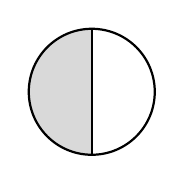
\begin{tikzpicture}[baseline=-0.5ex]
\fill[gray!30] (0,0) -- (0,0.8) arc (90:270:0.8cm) -- cycle;
\draw[thick] (0,0) circle (0.8cm);
\draw[thick] (0,0.8) -- (0,-0.8);
\end{tikzpicture} & &
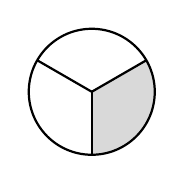
\begin{tikzpicture}[baseline=-0.5ex]
\fill[gray!30] (0,0) -- ++(270:0.8cm) arc (270:390:0.8cm) -- cycle;
\draw[thick] (0,0) circle (0.8cm);
\foreach \angle in {270,30,150}
    \draw[thick] (0,0) -- ++(\angle:0.8cm);
\end{tikzpicture} & &
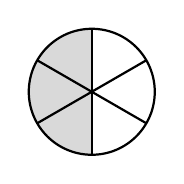
\begin{tikzpicture}[baseline=-0.5ex]
\fill[gray!30] (0,0) -- (0,0.8) arc (90:270:0.8cm) -- cycle;
\draw[thick] (0,0) circle (0.8cm);
\foreach \angle in {90,150,210,270,330,30}
    \draw[thick] (0,0) -- ++(\angle:0.8cm);
\end{tikzpicture} & &
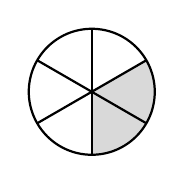
\begin{tikzpicture}[baseline=-0.5ex]
\fill[gray!30] (0,0) -- ++(270:0.8cm) arc (270:390:0.8cm) -- cycle;
\draw[thick] (0,0) circle (0.8cm);
\foreach \angle in {90,150,210,270,330,30}
    \draw[thick] (0,0) -- ++(\angle:0.8cm);
\end{tikzpicture} & &
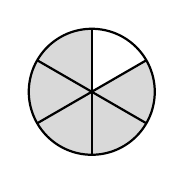
\begin{tikzpicture}[baseline=-0.5ex]
\fill[gray!30] (0,0) -- (0,0.8) arc (90:390:0.8cm) -- cycle;
\draw[thick] (0,0) circle (0.8cm);
\foreach \angle in {90,150,210,270,330,30}
    \draw[thick] (0,0) -- ++(\angle:0.8cm);
\end{tikzpicture} \\[5ex]
$\displaystyle\frac{1}{\rbox{2}}$ & $+$ & $\displaystyle\frac{1}{\bbox{3}}$ & $=$ & $\displaystyle\frac{1\times\bbox{3}}{\rbox{2}\times\bbox{3}}$ & $+$ & $\displaystyle\frac{1\times\rbox{2}}{\bbox{3}\times\rbox{2}}$ & $=$ & $\displaystyle\frac{5}{6}$ \\[3.5ex]
$\displaystyle\frac{1}{2}$ & $+$ & $\displaystyle\frac{1}{3}$ & $=$ & $\displaystyle\frac{3}{6}$ & $+$ & $\displaystyle\frac{2}{6}$ & $=$ & $\displaystyle\frac{5}{6}$
\end{tabular}
\end{center}
\end{itemize}

\begin{exercises}
\item
Add the missing numbers to calculate $\frac{3}{4}-\frac{2}{3}$. 
\begin{center}
\begin{tabular}{ccccccccccc}
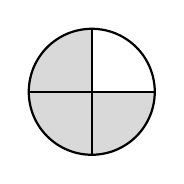
\begin{tikzpicture}[baseline=-0.5ex]
\fill[gray!30] (0,0) -- (0,0.8) arc (90:360:0.8cm) -- cycle;
\draw[thick] (0,0) circle (0.8cm);
\draw[thick] (0,0.8) -- (0,-0.8);
\draw[thick] (-0.8,0) -- (0.8,0);
\end{tikzpicture} & &
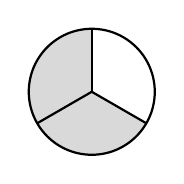
\begin{tikzpicture}[baseline=-0.5ex]
\fill[gray!30] (0,0) -- (0,0.8) arc (90:330:0.8cm) -- cycle;
\draw[thick] (0,0) circle (0.8cm);
\foreach \angle in {90,210,330}
    \draw[thick] (0,0) -- ++(\angle:0.8cm);
\end{tikzpicture} & &
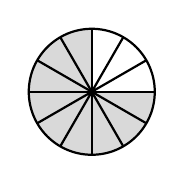
\begin{tikzpicture}[baseline=-0.5ex]
\fill[gray!30] (0,0) -- (0,0.8) arc (90:360:0.8cm) -- cycle;
\draw[thick] (0,0) circle (0.8cm);
\foreach \angle in {90,120,150,180,210,240,270,300,330,0,30,60}
    \draw[thick] (0,0) -- ++(\angle:0.8cm);
\end{tikzpicture} & &
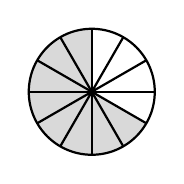
\begin{tikzpicture}[baseline=-0.5ex]
\fill[gray!30] (0,0) -- (0,0.8) arc (90:330:0.8cm) -- cycle;
\draw[thick] (0,0) circle (0.8cm);
\foreach \angle in {90,120,150,180,210,240,270,300,330,0,30,60}
    \draw[thick] (0,0) -- ++(\angle:0.8cm);
\end{tikzpicture} & &
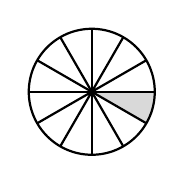
\begin{tikzpicture}[baseline=-0.5ex]
\fill[gray!30] (0,0) -- (0.8,0) arc (0:-30:0.8cm) -- cycle;
\draw[thick] (0,0) circle (0.8cm);
\foreach \angle in {90,120,150,180,210,240,270,300,330,0,30,60}
    \draw[thick] (0,0) -- ++(\angle:0.8cm);
\end{tikzpicture} \\[5ex]
$\displaystyle\frac{3}{\rbox{4}}$ & 
$-$ & $\displaystyle\frac{2}{\bbox{3}}$ & 
$=$ & $\displaystyle\frac{3\times\bbox{\phantom{3}}}{\rbox{\phantom{4}}\times\bbox{\phantom{3}}}$ & 
$-$ & $\displaystyle\frac{2\times\rbox{\phantom{4}}}{\bbox{\phantom{3}}\times\rbox{\phantom{4}}}$ & 
$=$ & $\displaystyle\frac{\hide{1}}{\hide{12}}$ \\[3.5ex]
$\displaystyle\frac{3}{4}$ & 
$-$ & $\displaystyle\frac{2}{3}$ & 
$=$ & $\displaystyle\frac{\hide{9}}{\hide{12}}$ & 
$-$ & $\displaystyle\frac{\hide{8}}{\hide{12}}$ & 
$=$ & $\displaystyle\frac{\hide{1}}{\hide{12}}$
\end{tabular}
\end{center}
\item
Without drawing pizzas, calculate
$$
\text{a)}\quad \frac{1}{4}+\frac{1}{3},\quad\quad \text{b)}\quad \frac{4}{5} + \frac{2}{3}, \quad\quad \text{c)}\quad \frac{5}{6}-\frac{1}{5}, \quad\quad \text{d)}\quad \frac{5}{8} + \frac{7}{12}.
$$
\end{exercises}

\section{Fractions and the Least Common Multiple}
\begin{itemize}
\item
When calculating expressions like 
$$\frac{1}{8} + \frac{1}{12},$$ 
using the common multiple $8\times 12 = 96$ produces a large denominator! Instead, we can use the \underbar{least common multiple}. First, find the \underbar{prime factors} of $8$ and $12$.
\begin{center}
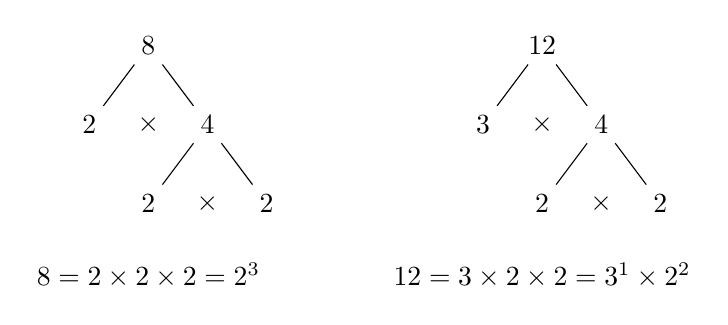
\begin{tikzpicture}[
  style={sibling distance=1.5cm, level distance=1cm},
]
  % First tree for 8
  \node (root2) {$8$}
    child {node (e) {$2$}}
    child {node (f) {$4$}
        child {node (g) {$2$}}
        child {node (h) {$2$}}
    };
    \path (e) -- node[midway] {$\times$} (f);
    \path (g) -- node[midway] {$\times$} (h);
    \node[below=.4cm of g] {$8 = 2 \times 2 \times 2 = 2^3$};

    % Second tree for 12
\begin{scope}[xshift=5cm]
    \node (root) {$12$}
    child {node (a) {$3$}}
    child {node (b) {$4$}
      child {node (c) {$2$}}
      child {node (d) {$2$}}
    };
    \path (a) -- node[midway] {$\times$} (b);
    \path (c) -- node[midway] {$\times$} (d);
    \node[below=.4cm of c] {$12 = 3 \times 2 \times 2 = 3^1\times 2^2$};
\end{scope}
\end{tikzpicture}
\end{center}
\vspace{-1em}
So $8=2^3$ and $12=2^2\times 3^1$. The least common multiple is $2^3\times 3^1 = 24$. Notice that $8\times \rbox{3} = 24$ and $12\times \bbox{2} = 24$, so
\begin{align*}
\frac{1}{8}+\frac{1}{12} &= \frac{1\times \rbox{3}}{8 \times \rbox{3}}+\frac{1 \times \bbox{2}}{12\times \bbox{2}} \\
&= \frac{3}{24} + \frac{2}{24} = \frac{5}{24}.
\end{align*}
\end{itemize}

\begin{exercises}
\item
Add the missing numbers to calculate $\frac{7}{18}-\frac{5}{27}$. To find the least common multiple, first find the prime factors of $18$ and $27$.
\begin{center}
\begin{tikzpicture}[
  style={sibling distance=1.5cm, level distance=1cm},
]
  % First tree for 18
  \node (root1) {$18$}
    child {node (a1) {$2$}}
    child {node (b1) {$\hide{9}$}
        child {node (c1) {$3$}}
        child {node (d1) {$3$}}
    };
    \path (a1) -- node[midway] {$\times$} (b1);
    \path (c1) -- node[midway] {$\times$} (d1);
    \node[below=.4cm of c1] {$18 = 2 \times 3 \times 3 = 2^1\times 3^2$};

    % Second tree for 27
\begin{scope}[xshift=6.5cm]
    \node (root2) {$27$}
    child {node (a2) {$3$}}
    child {node (b2) {$\hide{9}$}
      child {node (c2) {$3$}}
      child {node (d2) {$\hide{3}$}}
    };
    \path (a2) -- node[midway] {$\times$} (b2);
    \path (c2) -- node[midway] {$\times$} (d2);
    \node[below=.4cm of c2] {$27 = 3 \times 3 \times \hide{3} = \hide{3^3}$};
\end{scope}
\end{tikzpicture}
\end{center}
\vspace{-1em}
So $18=2^1\times 3^2$ and $27=\hide{3^3}$. The least common multiple is $\hide{2^1}\times \hide{3^3} = 54$. Notice that $18\times \rbox{\phantom{3}} = 54$ and $27\times \bbox{\phantom{2}} = 54$, so
\begin{align*}
\frac{7}{18}-\frac{5}{27} &= \frac{7\times \rbox{\phantom{3}}}{18 \times \rbox{\phantom{3}}}-\frac{5 \times \bbox{\phantom{2}}}{27\times \bbox{\phantom{2}}} \\
&= \frac{\hide{21}}{54} - \frac{\hide{10}}{54} = \frac{\hide{11}}{54}.
\end{align*}
\item
Find the least common multiple of the denominators to calculate
$$
\text{a)}\quad \frac{1}{6}+\frac{3}{8},\quad\quad \text{b)}\quad \frac{4}{5}-\frac{1}{10},\quad\quad \text{c)}\quad \frac{3}{12} + \frac{5}{16},\quad\quad \text{d)}\quad \frac{27}{32} - \frac{7}{24}.
$$
\end{exercises}

\bibliographystyle{ametsocV6}
\bibliography{references}

\end{document}